\documentclass[11pt, oneside]{article}   	% use "amsart" instead of "article" for AMSLaTeX format
\usepackage{geometry}                		% See geometry.pdf to learn the layout options. There are lots.
\geometry{letterpaper}                   		% ... or a4paper or a5paper or ... 
%\geometry{landscape}                		% Activate for for rotated page geometry
%\usepackage[parfill]{parskip}    		% Activate to begin paragraphs with an empty line rather than an indent
\usepackage{graphicx}				% Use pdf, png, jpg, or eps§ with pdflatex; use eps in DVI mode
								% TeX will automatically convert eps --> pdf in pdflatex		
\usepackage{amssymb}
\usepackage{amsmath}
\usepackage{parskip}
\usepackage{color}
\usepackage{hyperref}

\title{Shell Theorem}
%\author{The Author}
%\section{}
%\subsection*{}
\date{}							% Activate to display a given date or no date

\graphicspath{{/Users/telliott_admin/Dropbox/Tex/png/}}
% \begin{center} 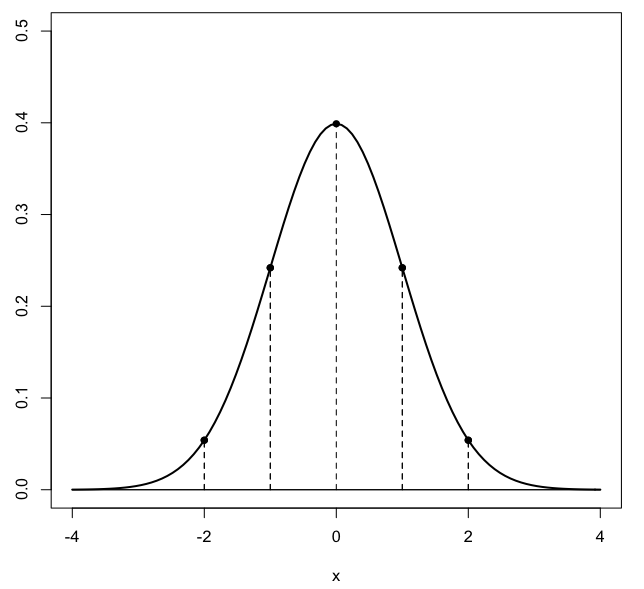
\includegraphics [scale=0.4] {gauss3.png} \end{center}
\begin{document}
\maketitle
\Large
Wikipedia has a beautiful derivation of the "shell theorem," which says that the mass of a spherical object acts in gravitation as if the entire mass $M$ were concentrated at the center.

\large
\url{http://en.wikipedia.org/wiki/Shell_theorem}
\Large

In this write-up, we will show that this is true for a shell of radius $R$.  Having done that, if we visualize the solid ball as a series of concentric shells, we will have the full theorem.
\begin{center} 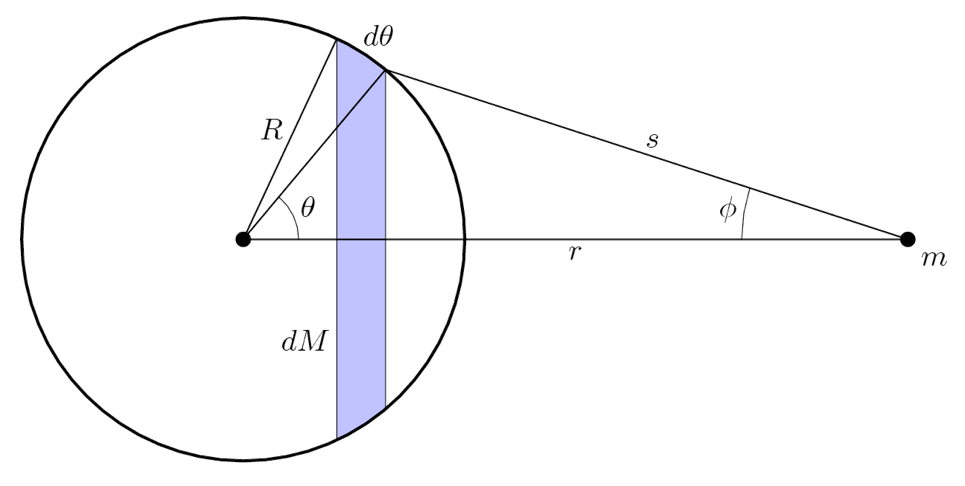
\includegraphics [scale=0.35] {shell_thm.png} \end{center}
The figure shows a cross-section of the shell.

We start by calculating the force due to a ring of mass contained inside the angular width $d \theta$, measured from the center of the shell

Using $\theta$ as the variable here is a great idea, because the mass is proportional to the area of the shell along this ring, and the width of the slice is $R \ d \theta$.

The radius of the ring is $R \sin \theta$, so the total surface area is
\[ dA = 2 \pi R \sin \theta R \ d \theta \]

The mass per unit area is the total mass $M$, divided by the surface area of the sphere
\[ \frac{M}{4 \pi R^2} \]
so the mass of the ring is the mass per unit area times the area for the ring
\[ M_r = \frac{M}{4 \pi R^2} \ 2 \pi R \sin \theta R \ d \theta \]
\[ = \frac{M}{2} \sin \theta \ d \theta \]

Each small piece of the ring has mass $dM$ and lies at a distance $s$ from the test mass $m$.
\begin{center} 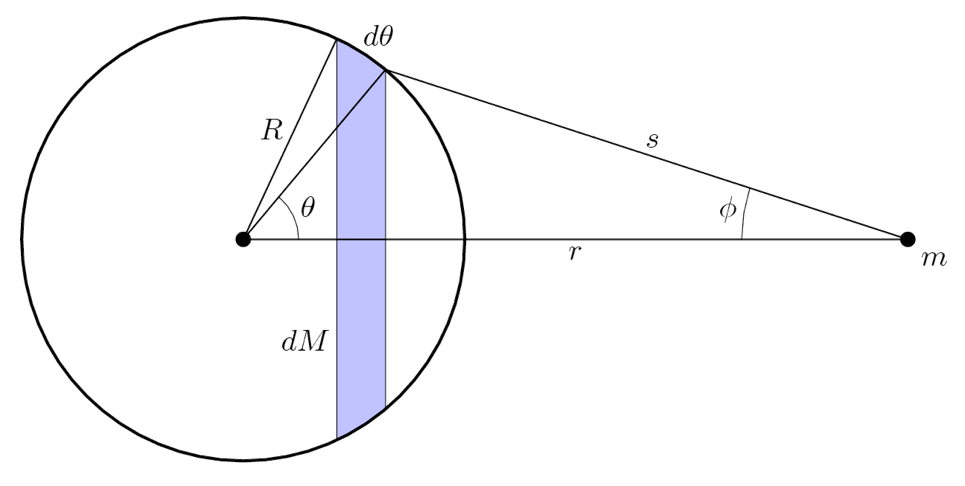
\includegraphics [scale=0.35] {shell_thm.png} \end{center}
It exerts a force of 
\[ dF = \frac{m G \ dM}{s^2} \]

The second critical insight is that for each piece the force has two components.  One acts along a line from the center of the sphere.

The other component cancels, because on the opposite side of the ring there is another small piece with the same force, but in the opposite direction.

The magnitude of the radial part is
\[ dF_r = dF \cos \phi = \frac{mG \cos \phi}{s^2} \ dM \]

(the force points toward the center of the shell, but in what follows I will work just with the magnitude.  You can pretend there is a unit radial vector coming along in all the calculations).

The total radial force is obtained by substituting the mass of the ring
\[ dF_r = \frac{mG \cos \phi}{s^2} \ \frac{M}{2} \sin \theta \ d \theta \]
\[ = \frac{GmM}{2} \frac{1}{s^2} \ \cos \phi \sin \theta \ d \theta \]

We should integrate from $\theta = 0 \rightarrow \pi$ to get the whole thing.

\subsection*{law of cosines}
While the above equation sounds nice, the trouble is that it contains three variables:  $s, \phi$, and $\theta$.  

However, the law of cosines will come to the rescue.  We write two formulas:

\[ R^2 = s^2 + r^2 - 2rs \cos \phi \]
\[ \cos \phi = \frac{s^2 + r^2 - R^2}{2rs} \]
and
\[ s^2 = R^2 + r^2 - 2rR \cos \theta \]
\[ \cos \theta = \frac{R^2 + r^2 - s^2}{2rR} \]

We need $\sin \theta$.  Differentiate the second equation (implicitly)
\[ -\sin \theta \ d \theta = -\frac{2s}{2rR} \ ds  \]
\[ \sin \theta \ d \theta = \frac{s}{rR} \ ds \]

The equation that we had was
\[ dF_r = \frac{GmM}{2} \frac{1}{s^2} \ \cos \phi \sin \theta \ d \theta \]

substitute for $\sin \theta \ d \theta$
\[ dF_r = \frac{GmM}{2} \frac{1}{s^2} \ \cos \phi \ \frac{s}{rR} \ ds \]
substitute for $\cos \phi$
\[ dF_r = \frac{GmM}{2} \ \frac{1}{s^2} \ \frac{(s^2 + r^2 - R^2)}{2rs} \ \frac{s}{rR} \ ds \]
\[ =  \frac{GmM}{4R r^2} \ \frac{(s^2 + r^2 - R^2)}{s^2} \ ds \]
\[ =  \frac{GmM}{4R r^2} \ (1 + \frac{(r^2 - R^2)}{s^2}) \ ds \]

The integral is
\[ F_r = \int dF_r = \int \frac{GmM}{4R r^2} \ (1 + \frac{(r^2 - R^2)}{s^2}) \ ds \]
\[ =  \frac{GmM}{4R r^2} \ [ \ s -  \frac{(r^2 - R^2)}{s}) \ ]  \]

What about the limits on $s$?  When $\theta = 0$, $s = r - R$, and when $\theta = \pi$, $s = r + R$ so we have
\[ F_r = \frac{GmM}{4R r^2} \ [ \ s -  \frac{(r^2 - R^2)}{s}) \ ] \ \bigg |_{r - R}^{r +R} \]
Notice that we can factor $r^2 - R^2$
\[ F_r = \frac{GmM}{4R r^2} \ [ \ s -  \frac{(r+R)(r-R)}{s}) \ ] \ \bigg |_{r - R}^{r +R} \]
So, just looking at the part in the brackets, at the upper limit we have
\[ r + R - (r - R) = 2R \]
at the lower limit
\[ r - R - (r + R) = -2R \]
doing the subtraction 
\[ = 4R \]
and $4R$ just cancels!  We obtain
\[ F_r = \frac{GmM}{r^2} \]

\end{document}  